%%%%%%%%%%%%%%%%%%%%%%%%%%%%%%%%%%%%%%%%%%%%%%%%%%%%%%%
%                   File: OSAmeetings.tex             %
%                  Date: March 21, 2007  MSD          %
%                                                     %
%     For preparing LaTeX manuscripts for submission  %
%       submission to OSA meetings and conferences    %
%                                                     %
%       (c) 2007 Optical Society of America           %
%%%%%%%%%%%%%%%%%%%%%%%%%%%%%%%%%%%%%%%%%%%%%%%%%%%%%%%

\documentclass[letterpaper,10pt]{article}
\usepackage{osameet2}

%% standard packages and arguments should be modified as needed

\usepackage{amsmath, amssymb}
\usepackage{graphicx}
%\usepackage[caption=false]{subfig}
\usepackage{caption}
\usepackage{braket}
\usepackage{siunitx}
\captionsetup{width=6in}
\usepackage[utf8]{inputenc}
\usepackage[T1]{fontenc}
\usepackage{subcaption}
\usepackage{pdfpages}
%\usepackage{cleveref}
\usepackage[pdftex,colorlinks=true,bookmarks=false,linkcolor=black,citecolor=blue,urlcolor=blue]{hyperref} %pdflatex
%\usepackage[dvips,colorlinks=true,bookmarks=false,citecolor=blue,urlcolor=blue]{hyperref} %latex w/dvips


\begin{document}

\title{From 2-Qubit Measurement Based Probabilistic Entangling Gate to Cluster States}

%\author{Xiruo Yan$^{1,2}$*, Jingda Wu$^{1,2}$, Ryan C. Watt$^1$, Megan K. T.  Nantel$^1$, Lukas Chrostowski$^{2,3}$ and Jeff F. Young$^{1,2}$}
\section{Spec sheet}
\label{spec}
We build a quantum computer architecture from the following building blocks:
\begin{enumerate}
\item A deterministic or probabilistic entangling gate for matter qubits, involving the preparation of certain photon states (single-photon states or less complicated), photon-matter qubit interaction, and photon detection.
\item One-qubit unitary gates on the matter qubits
\item One-qubit measurements on the matter qubit
\item Fast switching and routing of photons
\end{enumerate}

\section{Dipole-induced transparency entangling scheme}
\label{sec:DIT}
The schematics is shown as in figure \ref{fig:schematics}. I tried to follow the same labelling as in \cite{Sridharan2008} for WG field operators, but I have included the source input port ($s_{in}$), an extra beamspliter (bottom one) and 2 more detectors ($d_3$ and $d_4$). \\

\begin{figure}[h]
\centering
         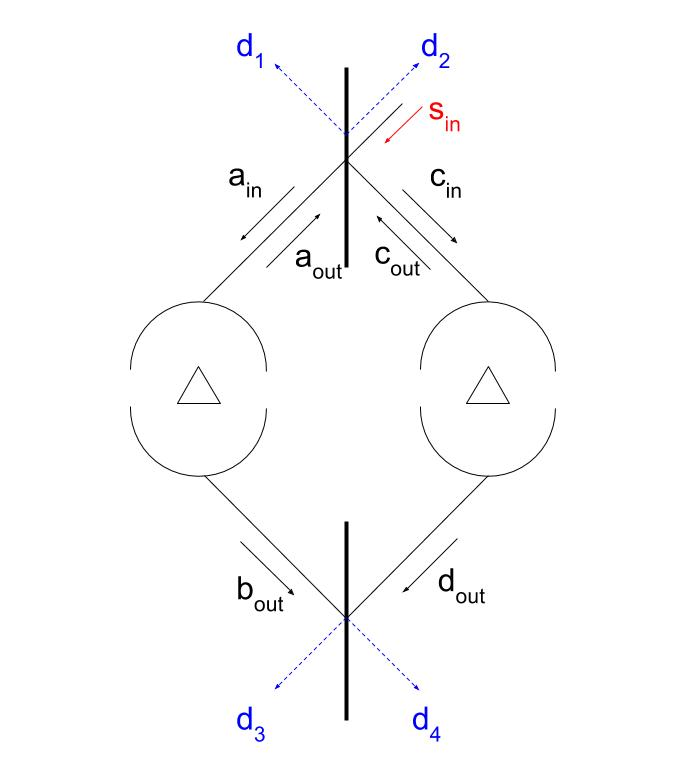
\includegraphics[width=2.5in]{DIT_entanglement.jpg}
         \caption{$s_{in}$ (red) is the source input port. $d_1\sim d_4$ (blue) are the detectors. }
         \label{fig:schematics}
\end{figure}

Two ground states of a qubit are $\Ket{g}$ and $\Ket{m}$, where $\Ket{g}$ is on resonance with the optical transition. Assume perfectly identical qubits, cavities and 50-50 beamspliters, there are following transformations: i) for BS I still follow the transformation in \cite{Sridharan2008}, which is the same as the \href{https://en.wikipedia.org/wiki/Hong%E2%80%93Ou%E2%80%93Mandel_effect}{HOM wiki page} ii) for dipole induced transparency I follow the transformation in \cite{Waks2006}:

\begin{align*}
%	s_{in}^\dag&\rightarrow\frac{1}{\sqrt{2}}(a_{in}^\dag+c_{in}^\dag)\quad (\textrm{first BS})\\
	a_{out}^\dag&\rightarrow\frac{1}{\sqrt{2}}(d_1^\dag+d_2^\dag)\quad (\textrm{first BS})\\
	c_{out}^\dag&\rightarrow\frac{1}{\sqrt{2}}(d_1^\dag-d_2^\dag)\quad (\textrm{first BS})\\
	a_{in}^\dag&\rightarrow a_{out}^\dag\quad (\textrm{left qubit in} \Ket{g})\\
	a_{in}^\dag&\rightarrow b_{out}^\dag\quad (\textrm{left qubit in} \Ket{m})
\end{align*}

%Some confusions on these transformations so far: 
%\begin{itemize}
%\item
%It seems the BS here is modelled in a different way as you showed (no imaginary part in the transformation)?
%\item  
%With the above BS convention, does $s_{in}^\dag\rightarrow\frac{1}{\sqrt{2}}(a_{in}^\dag+c_{in}^\dag)$ follow?
%\item
%I understood dipole induced transparency in a photon blockade picture, but how does a single photon get 100\% reflected when it meets the dipole in cavity?
%\item
%For the last equation above, \cite{Waks2006} (where QD cavity treated as drop a filter) used $a_{out}^\dag\rightarrow -b_{out}^\dag$, where does the phase shift come from?
%\end{itemize}
\subsection{The ideal case}
\label{subsec:DIT_ideal}
Starting with the \textbf{most ideal} case where the 2 qubits are prepared in the state $1/\sqrt{2}(\Ket{g}+\Ket{m})$, and a single photon in the input port $s_{in}$, the system state:
\begin{align*}
	\Ket{\psi_{sys}} &= \frac{\Ket{g}+\Ket{m}}{\sqrt{2}}\otimes\frac{\Ket{g}+\Ket{m}}{\sqrt{2}}\otimes s_{in}^\dag\Ket{0}\\
	\textrm{After the first BS}\quad &\rightarrow \frac{1}{2}(\Ket{gg}+\Ket{gm}+\Ket{mg}+\Ket{mm})\frac{1}{\sqrt{2}}(a_{in}^\dag+c_{in}^\dag)\Ket{0}\\
		%%%%%%
	\textrm{After 2 qubits}\quad &\rightarrow\frac{1}{2}[\Ket{gg}\frac{1}{\sqrt{2}}(a_{out}^\dag+c_{out}^\dag)\\
	&\quad\,+\Ket{gm}\frac{1}{\sqrt{2}}(a_{out}^\dag+d_{out}^\dag)\\
	&\quad\,+\Ket{mg}\frac{1}{\sqrt{2}}(b_{out}^\dag+c_{out}^\dag)\\
	&\quad\,+\Ket{mm}\frac{1}{\sqrt{2}}(b_{out}^\dag+d_{out}^\dag)]\\
	    %%%%%%
	\textrm{After mixing outputs at both BS}\quad &\rightarrow\frac{1}{2}[\Ket{gg}\frac{1}{\sqrt{2}}(\frac{d_1+d_2}{\sqrt{2}}+\frac{d_1-d_2}{\sqrt{2}})\\
	&\quad\,+\Ket{gm}\frac{1}{\sqrt{2}}(\frac{d_1+d_2}{\sqrt{2}}+\frac{d_3+d_4}{\sqrt{2}})\\
	&\quad\,+\Ket{mg}\frac{1}{\sqrt{2}}(\frac{d_3-d_4}{\sqrt{2}}+\frac{d_1-d_2}{\sqrt{2}})\\
	&\quad\,+\Ket{mm}\frac{1}{\sqrt{2}}(\frac{d_3-d_4}{\sqrt{2}}+\frac{d_3+d_4}{\sqrt{2}})]\\
	   %%%%%%
	&=\frac{1}{4}[(2\Ket{gg}+\Ket{gm}+\Ket{mg})d_1\\
	&\quad\,+(\Ket{gm}-\Ket{mg})d_2\\
	&\quad\,+(\Ket{gm}+\Ket{mg}+2\Ket{mm})d_3\\
	&\quad\,+(\Ket{gm}-\Ket{mg})d_4]\\
	   %%%%%%
	&=\frac{1}{\sqrt{6}}(2\Ket{gg}+\Ket{gm}+\Ket{mg})\otimes\sqrt{\frac{3}{8}}d_1\\
	&\quad\, +\frac{1}{\sqrt{2}}(\Ket{gm}-\Ket{mg})\otimes\frac{1}{\sqrt{8}}d_2\\
	&\quad\, +\frac{1}{\sqrt{6}}(\Ket{gm}+\Ket{mg}+2\Ket{mm})\otimes\sqrt{\frac{3}{8}}d_3\\
	&\quad\, +\frac{1}{\sqrt{2}}(\Ket{gm}-\Ket{mg})\otimes\frac{1}{\sqrt{8}}d_4
\end{align*}
Then we come to the conclusion that if a detection event happens at detector $d_2$ or $d_4$, we know that we have the 2 qubits in the state$1/\sqrt{2}(\Ket{gm}-\Ket{mg})$. Moreover, the total probability for projecting the 2 qubits to this state is $1/4$. Otherwise we end up in other states. 
%\section{Conclusion}
%We have demonstrated by simulation that our design of the small-V PhC cavity can achieve high tunability while preserving high Q. Our unique design and control scheme can benefit high-precision many integrated optics applications that require individual tuning of on-chip high-Q PhC.

%\begin{figure}[h]
%\centering
%        \includegraphics[width=1.5in]{_002}       
%        \caption{SEM image of a fabricated device, for proof-of-principle demonstration.}\label{fig:sem}
%\end{figure}
\subsection{Generalization}
\label{subsec:DIT_gen}
Choosing the computational basis: $\Ket{g}\equiv\Ket{0}=(1\quad 0)^T$ and $\Ket{m}\equiv\Ket{1} = (0\quad 1)^T$, consider the system state with two atoms arbitrarily initialized: 
\begin{equation*}
	\Ket{\psi_{sys}} = (\alpha_1\Ket{0}+\beta_1\Ket{1})\otimes(\alpha_2\Ket{0}+\beta_2\Ket{1})\otimes s_{in}^\dag\Ket{0}_{field},
\end{equation*}
subject to normalization conditions:
\begin{align*}
	|\alpha_1|^2+|\beta_1|^2&=1\\
	|\alpha_2|^2+|\beta_2|^2&=1	
\end{align*}
Carrying out the same reasoning as before, the final system state is:
\begin{align*}
	\Ket{\psi} \Rightarrow & 	\frac{1}{2} [(2\alpha_1\alpha_2\Ket{00}+\alpha_1\beta_2\Ket{01}+\beta_1\alpha_2\Ket{10})d_1\\
	&+(\alpha_1\beta_2\Ket{01}-\beta_1\alpha_2\Ket{10})d_2\\
	&+(\alpha_1\beta_2\Ket{01}+\beta_1\alpha_2\Ket{10}+2\beta_1\beta_2\Ket{11})d_3\\
	&+(\alpha_1\beta_2\Ket{01}-\beta_1\alpha_2\Ket{10})d_4]
\end{align*}
By normalizing the qubit states, the following table of outcomes can be obtained:
\begin{table}
\centering
\begin{tabular}{ | m{2.5cm} | m{7cm}| m{6cm} |@{}m{0pt}@{}} 
\hline
Detection Event & Resulting Qubit State & Outcome Probability & \\ [5pt] 
\hline
$d_1$ & $1/(2\sqrt{N_1})(2\alpha_1\alpha_2\Ket{00}+\alpha_1\beta_2\Ket{01}+\beta_1\alpha_2\Ket{10})$ & $N_1 = |\alpha_1\alpha_2|^2+1/4|\alpha_1\beta_2|^2+1/4|\beta_1\alpha_2|^2$ & \\[5pt]
\hline
$d_2$ & $1/(2\sqrt{N_{2}})(\alpha_1\beta_2\Ket{01}-\beta_1\alpha_2\Ket{10})$ & $N_{2} = 1/4|\alpha_1\beta_2|^2+1/4|\beta_1\alpha_2|^2$ & \\[5pt]
\hline
$d_3$ & $1/(2\sqrt{N_3})(\alpha_1\beta_2\Ket{01}+\beta_1\alpha_2\Ket{10}+2\beta_1\beta_2\Ket{11})$ & $N_3 = 1/4|\alpha_1\beta_2|^2+1/4|\beta_1\alpha_2|^2+|\beta_1\beta_2|^2$ & \\[5pt]
\hline
$d_4$ & $1/(2\sqrt{N_{4}})(\alpha_1\beta_2\Ket{01}-\beta_1\alpha_2\Ket{10})$ & $N_{4} = 1/4|\alpha_1\beta_2|^2+1/4|\beta_1\alpha_2|^2$ & \\[5pt]
\hline
\end{tabular}
\caption{The table of the measurement outcomes}
\label{tab:1}
\end{table}
The outcomes of detection event at $d_2$ or $d_4$ are identical, regardless of initial qubit states. Further, if a photon is detected in $d_2$ or $d_4$, the general 2-qubit states:
\begin{equation*}
	\Ket{\psi} = (\alpha_1\Ket{0}+\beta_1\Ket{1})\otimes(\alpha_2\Ket{0}+		\beta_2\Ket{1}),
\end{equation*}
will end up in the state:
\begin{equation*}
	\Ket{\psi'} = \alpha_1\beta_2\Ket{01}-\beta_1\alpha_2\Ket{10}.
\end{equation*}
Hence, there exists an operation $T$ such that: 

\begin{equation*}
	\Ket{\psi'}=T\Ket{\psi},
\end{equation*}
or in matrix representation (omitting the global normalization factor):

\begin{equation*}
	\begin{bmatrix}
		0\\ \alpha_1\beta_2 \\ -\beta_1\alpha_2 \\ 0
	\end{bmatrix} = 
	\begin{bmatrix}
		& & & &\\ & & & & \\ & & & & \\ & & & &
	\end{bmatrix}
	\begin{bmatrix}
		\alpha_1\alpha_2\\ \alpha_1\beta_2 \\ \beta_1\alpha_2 \\ \beta_1\beta_2
	\end{bmatrix} 	
\end{equation*}
By inspection, $T$ is simply:
\begin{equation} \label{eq:T}	
	T=
	\begin{bmatrix}
		0 &0 &0 &0\\ 0&1 &0 &0 \\ 0& 0& -1 &0 \\ 0&0 &0 &0
	\end{bmatrix}=
	Diag(0,1,-1,0)
\end{equation}
This operator is a projection operator followed by a unitary Pauli Z operation on the first qubit, i.e., 
\begin{equation} \label{eq:T_Pauli}
	T=Z_1(\frac{I-Z_1\otimes Z_2}{2}), 
\end{equation}
Similarly, the operators to the qubits corresponding to a click at $d_1$ and $d_3$ (denoted by $E_1$ and $E_3$ respectively) are:
\begin{align}
	\label{eq:E1}
	E_1 &= Diag(2,1,1,0)\\
	\label{eq:E3}
	E_3&= Diag(0,1,1,2)
\end{align}

\section{Creation of cluster states}
\label{sec:create_cluster}
This section is mainly taken from Robert's document, but with more derivation steps. 
\subsection{Stabilizer formalism}
For detailed information, refer to Chapter 10.5 of Nielsen and Chuang \cite{Nielsen2000}. This part only provides basic context for Robert's document.\\
The basic idea is to use operators to describe states space, instead of states themselves. For a given state $\Ket{\psi}$, if there exists an operator $M$ such that:
\begin{equation*}
	M\Ket{\psi} = \Ket{\psi},
\end{equation*} 
then we say that $M$ stabilizes $\Ket{\psi}$, for example, Pauli $Z$ stabilizes $\Ket{0}$. Further, if a set of operators $S$ form a group (closed under matrix multiplication), and define $V_S$ to be the set of n-qubit states stabilized by every element in $S$, then $V_S$ is the vector space stabilized by $S$ and $S$ is the stabilizer of space $V_S$. Usually $S$ can be described by only its generators for maximum compactness, since other stabilizer group elements can be obtained by multiplying the generators.
Here lists some useful facts in the language of stabilizers:\\ \\
\underline{Unitary Gates}. Suppose we apply a unitary operation $U$ to a vector space $V_S$ stabilized by the group $S$. Let $\Ket{\psi}$ be any element of $V_S$. Then for any element $g$ of $S$,
\begin{equation}
	U\Ket{\psi}=Ug\Ket{\psi}=UgU^{\dag}U\Ket{\psi}.
\end{equation}
Therefore, after the gate the state is stabilized by $UgU^{\dag}$.\\ \\
\underline{Projective Measurements}. If $g$ is an observable (usually a product of Pauli matrices) to be measured, and the system is assumed to be in a state $\Ket{\psi}$ with stabilizer $<g_1,g_2,...g_n>$, then there are two possibilities:
\begin{enumerate}
	\item
	$g$ commutes with every generator in the stabilizer.
	\item
	$g$ anti-commutes with one or more generators of the stabilizer. If $g$ anti-commute with, say, $g_1$ and $g_2$, it can be easily shown that $g$ commutes with $g_1g_2$. We can simply replace the generator $g_2$ by $g_1g_2$ in our list of generators for the stabilizer. Therefore, we can always reduce to the case that $g$ anti-commutes with only 1 generator.

\end{enumerate}
For the first case, $g_jg\Ket{\psi}=gg_j\Ket{\psi}=g\Ket{\psi}$. $g\Ket{\psi}$ is also stabilized by every generator, therefore it is in $V_S$ and is a multiple of $\Ket{\psi}$. Since $g^2=I$, $g\Ket{\psi}=\pm\Ket{\psi}$. As a result, either $g$ or $-g$ must be in the stabilizer.\\
For the second case ($g$ anti-commutes with $g_1$), the projectors are given by $g$ is $(I\pm g)/2$. Depending on the measurement outcome ($+1$ or $-1$), the resulting state will be $(I+g)\Ket{\psi}/\sqrt{2}$ or $(I-g)\Ket{\psi}/\sqrt{2}$. Therefore, the new stabilizer becomes $<g,g_2...,g_n>$ or $<-g,g_2,...,g_n>$ (note that either way $g_1$ has been kicked out of the new stabilizer due to anti-commutativity with the measurement).

\subsection{Deterministic creation of cluster states}
\label{subsec:dcc}
Here shows how to create an arbitrary long 1D cluster state, given the deterministic entangling measurement of the observable $Z_i\otimes Z_j$. The following argument is by induction \cite{rrdoc}:\\

Assume we already have a 1D cluster state with n qubits $\Ket{\psi(n)}$, stabilized by $K_1 = X_1\otimes Z_2$, $K_n = Z_{n-1} \otimes X_n$, and
\begin{equation}
	K_l=Z_{l-1}\otimes X_l\otimes Z_{l+1}, \quad l=2,3..,n-1.
\end{equation}
The procedure of adding the $(n+1)$th qubit to the chain deterministically consists of three steps:
\begin{enumerate}
	\item
	A qubit n + 1 is prepared in the state $\Ket{+}$, resulting in the state $\Ket{\psi(n)}\otimes\Ket{+}_{n+1}$. \\ \\
	The system now is stabilized by $K_1,..,K_n$ and $X_{n+1}$.
	
	\item
	The observable $Z_n\otimes Z_{n+1}$ is measured on the last two qubits. If the outcome is “-1” then the Pauli operator $X_{n+1}$ is applied to the last qubit. \\ \\
	After the first measurement, $K_1,..,K_{n-1}$ remain in the stabilizer, since they commute with the observable, while $K_n$ and $X_{n+1}$ are removed since they anti-commute with the observable. As described in the previews subsection, the product of the last two operator $\tilde{K_n}=k_n\otimes X_{n+1}=Z_{n-1} \otimes X_n\otimes X_{n+1}$ can then be added to the stabilizer because it commutes with the observable. Also, depending on the measurement outcome being "+1" or "-1", $Z_n\otimes Z_{n+1}$ or $-Z_n\otimes Z_{n+1}$ can be added to the stabilizer.\\
	If the outcome is "+1", the step is finished.\\
	If the outcome is "-1", by applying unitary $X_{n+1}$ gate, the stabilizer $-Z_n\otimes Z_{n+1}$ undergoes the transform (other stabilizers commute with $X_{n+1}$, hence not affected):
	\begin{equation}
		-Z_n\otimes Z_{n+1}\Rightarrow -Z_n\otimes (X_{n+1}Z_{n+1}X_{n+1})=Z_n\otimes Z_{n+1}.
	\end{equation}
	Therefore, after this step, the stabilizer of the system are:
	\begin{equation}
		K_1,..,K_{n-1},\, \textrm{and} \, Z_{n-1} \otimes X_n\otimes X_{n+1}, \, Z_n\otimes Z_{n+1}
	\end{equation}
	
	\item
	A Hadamard gate $H_{n+1}$ is applied to the last qubit.\\ \\
	By applying the Hadamard gate, the last two stabilizers undergo the transformations:
	\begin{align}
		Z_{n-1} \otimes X_n\otimes X_{n+1} &\Rightarrow Z_{n-1} \otimes X_n\otimes(H_{n+1}X_{n+1}H_{n+1}) = Z_{n-1} \otimes X_n\otimes Z_{n+1}\equiv K_n\\
		Z_n\otimes Z_{n+1} &\Rightarrow Z_{n}\otimes(H_{n+1}Z_{n+1}H_{n+1}) = Z_{n}\otimes X_{n+1}\equiv K_{n+1}.
	\end{align}	
	Hence, the original 1D cluster grows by 1 qubit.	
\end{enumerate} 

\subsection{Probabilistic creation of cluster states}
\label{subsec:pcc}
This subsection discuss the previous creation procedures in a probabilistic situation: we can only make a probabilistic heralded entangling measurement of the observable $Z_i \otimes Z_j$. The procedure assumes in-advance prepared cluster states of length $l$ (as opposed to the 1 $(n+1)$th qubit in the previews case), which carry a cost per piece of $C(l)$\cite{rrdoc}.\\
The procedure for extending a 1D cluster state is:
\begin{enumerate}
	\item 
	Put in place the existing $n$-qubit cluster state $\Ket{\psi(n)}$ (qubits $1,2,..,n$) and an in-advance prepared $l$-qubit cluster state $\Ket{\psi(l)}$ (qubits $n+1,..,n+l$). \\ \\
	The stabilizers at this step are $\{K_1,..,K_n\}$ and $\{K_{n+1},.., K_{n+l}\}$ for the two cluster states respectively, as defined in the same fashion as in the beginning of the section \ref{subsec:dcc}.
	
	\item 
	Measure the observable $Z_n \otimes Z_{n+1}$ (and the conditional Pauli roation), as illustrated in Figure \ref{fig:entangle}. \\ \\
	This step is same as procedure 2 in section \ref{subsec:dcc}). If the measurement succeeds, continue with step $3a$. If the measurement fails, continue
with step $3b$.

\begin{figure}[h]
\centering
         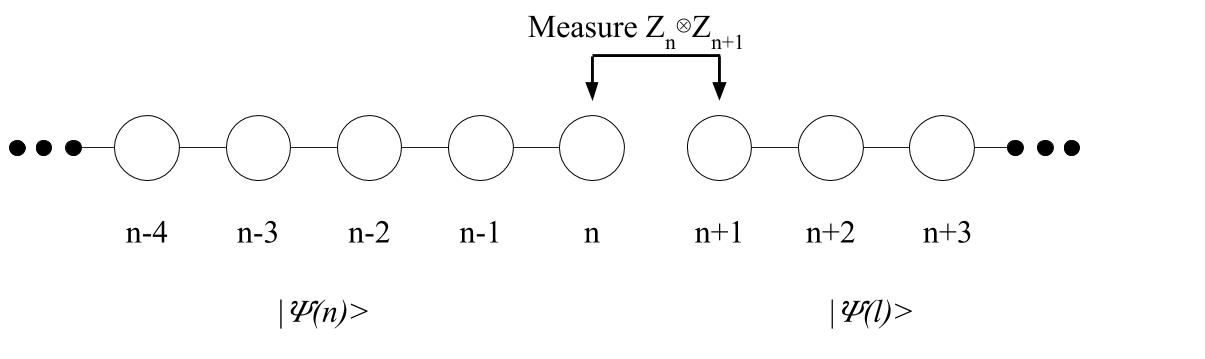
\includegraphics[height=1.2in]{entangling_1.jpg}
         \caption{Entangling 2 cluster states (conditional Pauli rotation omitted).}
         \label{fig:entangle}
\end{figure}

	\item[3a.]
	Measure the observable $X$ on the qubit $(n + 1)$. This results in a cluster state $\Ket{\psi(n+l-1)}$ of length $(n+l-1)$. \\ \\
	The stabilizers after a successful step 2 will then be:
	\begin{equation}
		K_1,..,K_{n-1},\,Z_{n-1}\otimes X_n\otimes X_{n+1}\otimes Z_{n+2},\, Z_n\otimes Z_{n+1}, \,K_{n+2},..,K_{n+l}.
	\end{equation}
	By measuring $X$ on the $(n+1)$th qubit, $Z_n\otimes Z_{n+1}$ and $K_{n+2}$ get kicked out of the stabilizer but their product $Z_n\otimes (Z_{n+1}Z_{n+1})\otimes X_{n+2}\otimes Z_{n+3}=Z_n\otimes X_{n+2}\otimes Z_{n+3}$ is added to the stabilizer. $X_{n+1}$ (assuming the measurement outcome is '+1') is also added to the stabilizer.\\
	Since $Z_{n-1}\otimes X_n\otimes X_{n+1}\otimes Z_{n+2}$ can be generated by $X_{n+1}$ and $Z_{n-1}\otimes X_n\otimes Z_{n+2}$, it can be replace by $Z_{n-1}\otimes X_n\otimes Z_{n+2}$ as a stabilizer.\\
	Therefore, after this step, stabilizers are:
	\begin{equation}
		K_1,..,K_{n-1},\,Z_{n-1}\otimes X_n\otimes Z_{n+2},\,Z_{n-1}\otimes X_n\otimes Z_{n+2},\,K_{n+3}..,K_{n+l}, \,\textrm{together with} \,\,X_{n+1}
	\end{equation}
	The net result it that the $(n+1)$th qubit is 'detached' from the system but the rest $(n+l-1)$ qubits form a cluster state, as illustrated in Figure \ref{fig:entangle_success}. If $l\gg 1$, the cluster state grows substantially.
	
	\item[3b.] Measure the observable $Z$ on qubit $n-1$, resulting in a cluster state $\Ket{\psi(n-2)}$ of length $n-2$.\\ \\
	Since the observable $Z_{n-1}$ commutes with the observable measured in step 2 $Z_n \otimes Z_{n+1}$, we can think of $Z_{n-1}$ as measured before the entangling gate in step 2.\\
	Starting with the stabilizers in step 1, since $K_{n-1}=Z_{n-2}\otimes X_{n-1}\otimes Z_n$ anti-commutes with $Z_{n-1}$, it is removed from the stabilizer. $ Z_{n-1}$ is added to the stabilizer. \\
	Also, we can replace $K_n = Z_{n-1}\otimes X_n$ with $X_n$ because it can be generated by $ Z_{n-1}$ and $X_n$. Similarly, $K_{n-2} = Z_{n-3}\otimes X_{n-2}\otimes Z_{n-1}$ can be replaced by $Z_{n-3}\otimes X_{n-2}$. The resulting stabilizers for $\Ket{\psi(n)}$ are:
	\begin{equation}
		K_1,..,K_{n-3}, K_{n-2} (\equiv Z_{n-3}\otimes X_{n-2}), Z_{n-1}, X_n
	\end{equation}
	The net result is that the $(n-1)$th and the $n$th qubits are 'detached' from $\Ket{\psi(n)}$. Hence the 'following' step 2 (which actually happens before measuring $Z_{n-1}$) will not affect the cluster state $\Ket{\psi(n-2)}$. In a word, this step sacrifices the last 2 qubits of $\Ket{\psi(n)}$ to save the rest of the entanglement from a failed entangling gate, as illustrated in Figure \ref{fig:entangle_failure}.
\end{enumerate}

\begin{figure}[htp]
\centering
    \begin{subfigure}[t]{0.5\textwidth}
        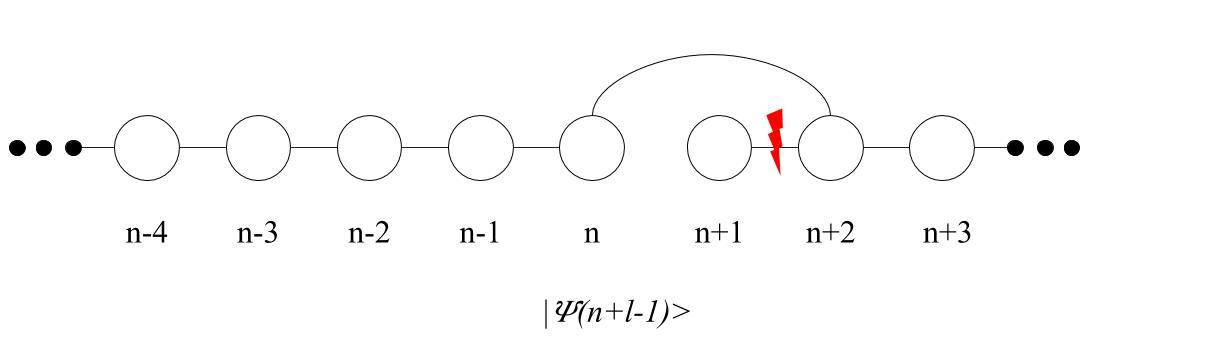
\includegraphics[height=1.2in]{entangling_2.jpg}
        \caption{Net result after 3(a)}
        \label{fig:entangle_success}
    \end{subfigure}%
    \\ 
    \begin{subfigure}[t]{0.5\textwidth}
        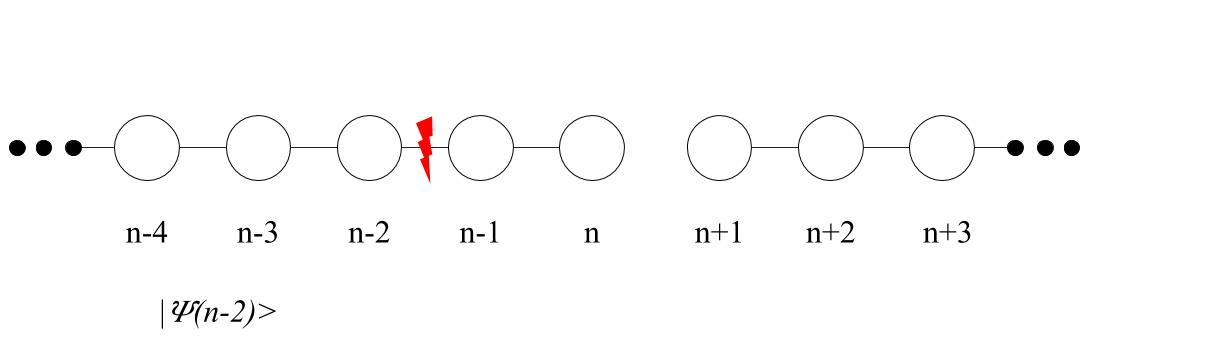
\includegraphics[height=1.2in]{entangling_3.jpg}
        \caption{Net result after 3(b)}
        \label{fig:entangle_failure}
    \end{subfigure}%
\caption{Illustrations for the step 3 in the probabilistic creation of cluster states}

\end{figure}

\section{Improving the photonic entangling gate}
Some natures of the entangling schemes described in section \ref{sec:DIT} can be used to improve the creation of the cluster states explained in section \ref{sec:create_cluster}.
\subsection{Iteration 1}
\label{subsec:iteration1}
From equations \ref{eq:T} - \ref{eq:E3}, we observe:
\begin{enumerate}
	\item 
	$E_1$ and $E_3$ commute with local $Z$-measurements on the two qubits they act on. This implies that the damage to the existing cluster state in case of gate failure is cut in half. \\ \\
	Therefore, at the 3b step in section \ref{subsec:pcc}, instead of measuring $Z$ on qubit $n-1$, we can simply measure $Z$ on qubit $n$, resulting in an $(n-1)$-qubit state $\Ket{\psi(n-1)}$, thus saving one qubit from the failed entangling gate, as shown in Figure \ref{fig:entangle_failure_improve}.
	\begin{figure}[h]
	\centering
         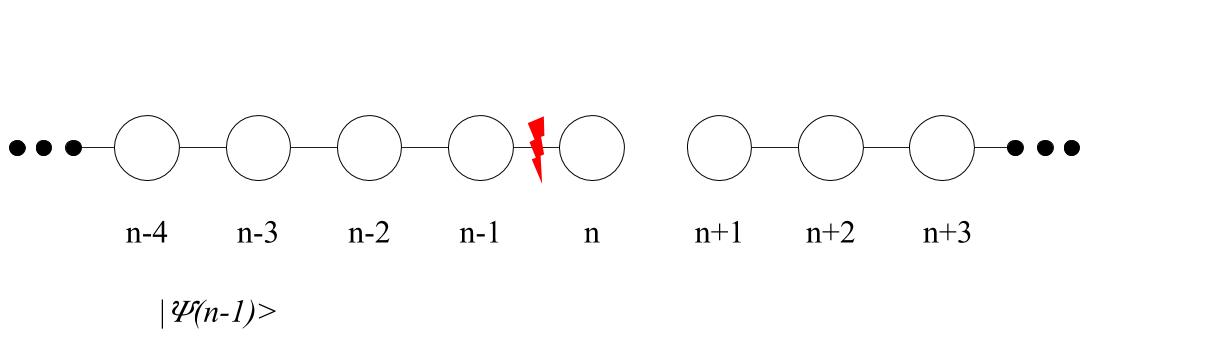
\includegraphics[height=1.2in]{entangling_4.jpg}
         \caption{Saving one qubit (compared to Figure \ref{fig:entangle_failure})}
         \label{fig:entangle_failure_improve}
	\end{figure}
	
	\item
	$E_1$ and $E_3$ commute also with the successful gate operation $T$, and we also have $E_{1/3}T=TE_{1/3}=T$. Thus, if we don’t like the outcome, we can measure \emph{again}. Namely,
	\begin{equation*}
		TE_1\sim E_1E_3\sim E_1T\sim E_3T\sim E_1E_2E_3\sim ... \sim T.
	\end{equation*}
	Thus, $(2, 1)$, i.e. outcome 1 followed by outcome 2, $(3, 1)$, $(1, 3)$, $(3, 3, 1)$, ... are all successful outcomes. Thus the success probability increases from $1/4$ to $1/2$.
\end{enumerate}
\subsection{Iteration 2}
\label{subsec:iteration2}
If an additional $50/50$ beam splitter is added to the original entangling scheme, as shown in Figure \ref{fig:schematics_2} \cite{rrdoc},
\begin{figure}[h]
\centering
         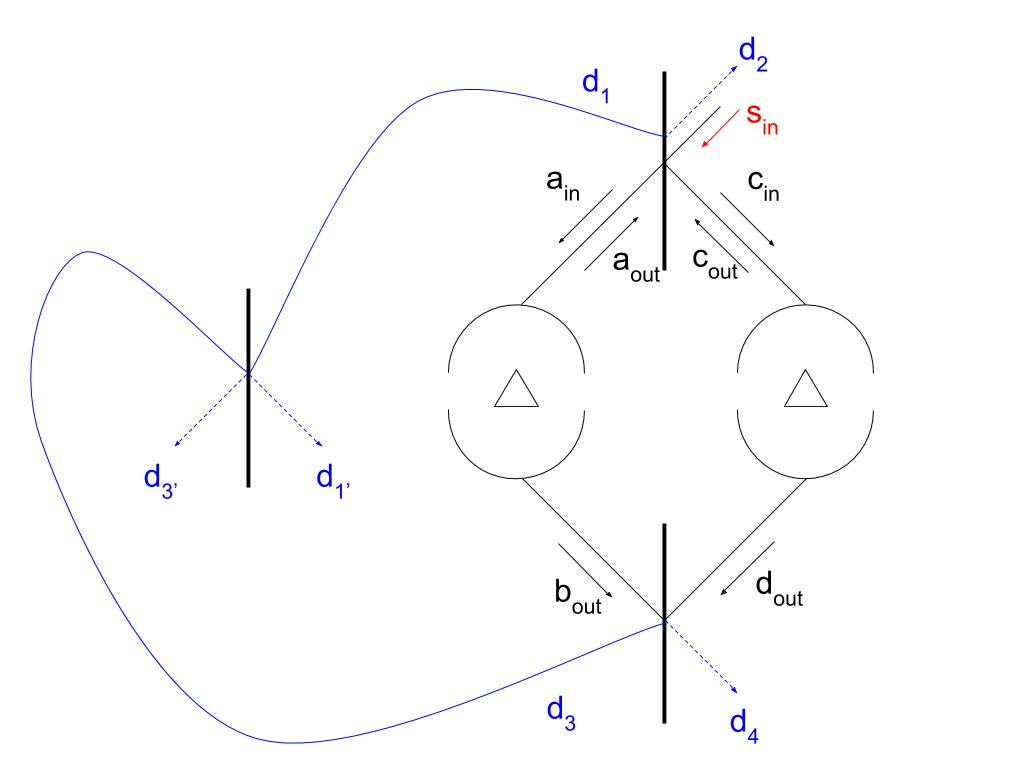
\includegraphics[width=3.5in]{DIT_entanglement_2.jpg}
         \caption{The outputs from $d_1$ and $d_3$ is combined at another beam splitter.}
         \label{fig:schematics_2}
\end{figure}
the final state will be (for the ideal case):
\begin{equation}
\begin{aligned}
	\Ket{\psi}&=\frac{1}{2}(\Ket{00}+\Ket{01}+\Ket{10}+\Ket{11})\otimes \frac{1}{\sqrt{2}}d_{1'}\\
	&\quad\, +\frac{1}{\sqrt{2}}(\Ket{01}-\Ket{10})\otimes\frac{1}{\sqrt{8}}d_2\\
	&\quad\, +\frac{1}{\sqrt{2}}(\Ket{00}-\Ket{11})\otimes\frac{1}{2}d_{3'}\\
	&\quad\, +\frac{1}{\sqrt{2}}(\Ket{01}-\Ket{10})\otimes\frac{1}{\sqrt{8}}d_4
\end{aligned}
\end{equation}
The operators corresponding to the detection event at $d_{1'}$ and $d_{3'}$ are then:
\begin{align}
	\label{eq:E1'}
	E_{1'} &= I \sim E_1+E_3\\
	\label{eq:E3'}	
	E_{3'} &= Diag(1,0,0,-1) \sim E_1-E_3 \sim Z_1\frac{I+Z_1\otimes Z_2}{2}
\end{align}
Similarly, as suggested by Jeff, if we combine the output of $d_2$ and $d_4$ with a beam splitter, arriving at a schematic shown in Figure \ref{fig:schematics_3}, we would have the outcome:
\begin{equation}
\begin{aligned}
	\Ket{\psi}&=\frac{1}{2}(\Ket{00}+\Ket{01}+\Ket{10}+\Ket{11})\otimes \frac{1}{\sqrt{2}}d_{1'}\\
	&\quad\, +\frac{1}{\sqrt{2}}(\Ket{01}-\Ket{10})\otimes\frac{1}{2}d_{2'}\\
	&\quad\, +\frac{1}{\sqrt{2}}(\Ket{00}-\Ket{11})\otimes\frac{1}{2}d_{3'}
\end{aligned}
\end{equation}
\begin{figure}[h]
\centering
         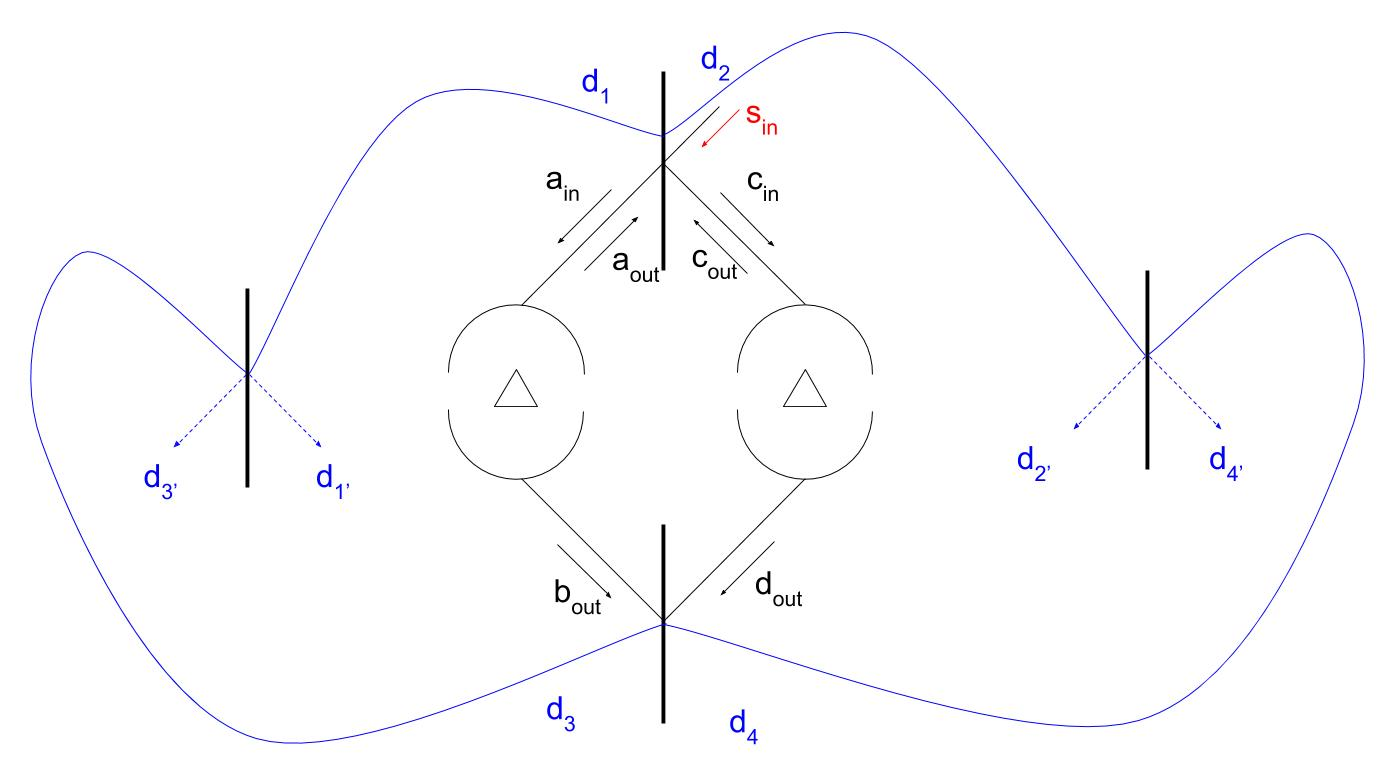
\includegraphics[width=5.5in]{DIT_entanglement_3.jpg}
         \caption{The outputs from $d_1$ and $d_3$ is combined at another beam splitter.}
         \label{fig:schematics_3}
\end{figure}

%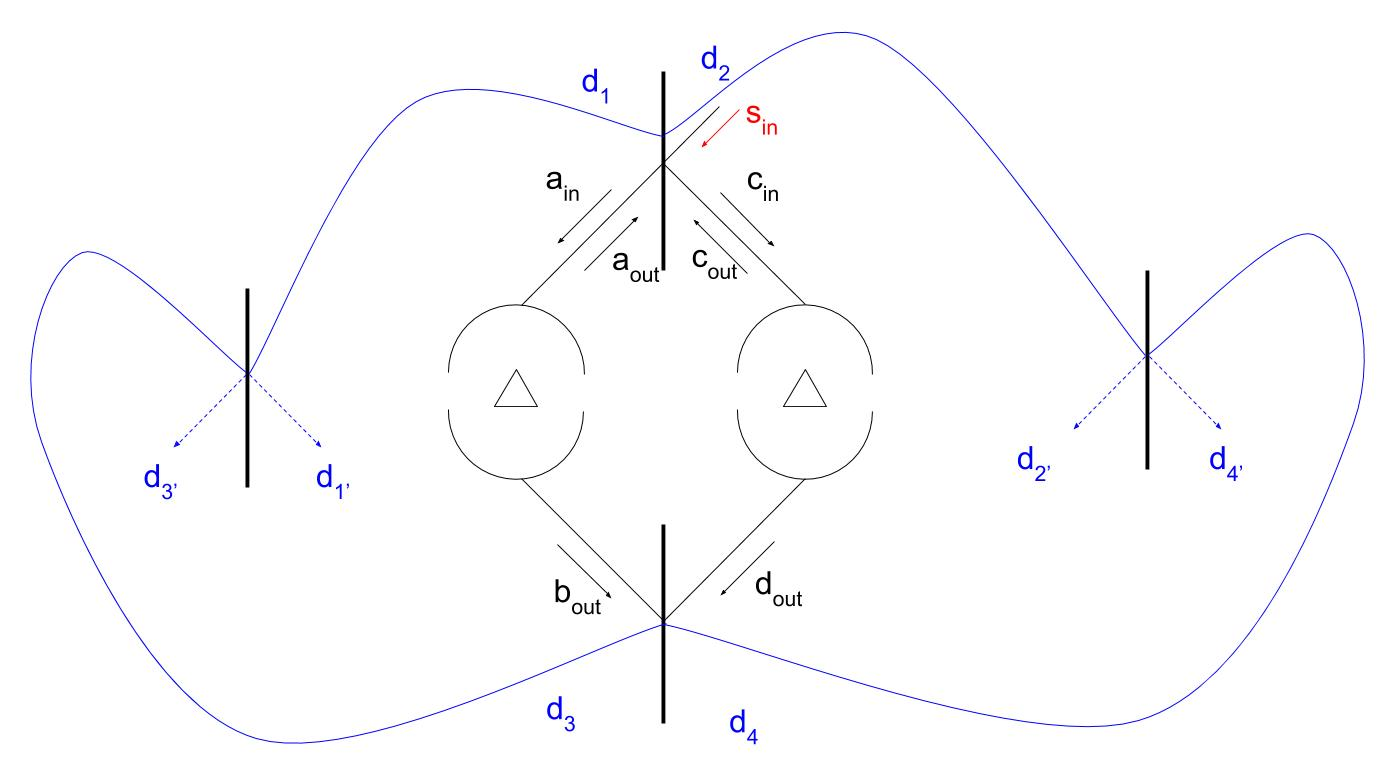
\includepdf[width=0.1\textwidth, angle = 90]{DIT_entanglement_3.pdf}
Therefore, no photon should be coming out of port $d_{4'}$, and we save a single photon detector ($d_{4'}$), and:
\begin{equation}
	\label{eq:E2'}
	E_{2'} =Diag(0,1,-1,0)\sim Z_1(\frac{I-Z_1\otimes Z_2}{2}).
\end{equation}

Note that in this scheme, it can be easily verified that the operators \ref{eq:E1'}, \ref{eq:E3'} and \ref{eq:E2'} are valid for any initial qubit states, since the interference of the photon does not depend on the qubit states. Only the success probability can be affected by the initial qubit states, in a way analogous to Table \ref{tab:1}.
%such that
%
%More notations: 
%\begin{itemize}
%	\item $I$ is the identity;
%	\item $X,\,Y,\,Z$ are Pauli matrices; 
%	\item The subscript indicates the the qubit on which the operator is acting on, for example with the 2-qubit case, $Z_1\equiv Z\otimes I$, $Z_1Z_2\equiv Z\otimes Z$, etc.
%	\item Superposition x-positive and x-negative states: $\Ket{\pm}=1/\sqrt{2}(\Ket{0}\pm\Ket{1})$.
%\end{itemize}
%The scheme to create a 1D chain of entangled qubits is shown as in Figure \ref{fig:1D_cluster}. The scheme goes as entangling the first 2 qubits, applying Hadamard gate on the 2nd qubit, entangling the 2nd and 3rd qubits, applying Hadamard gate on the 3rd qubit, entangling the 3rd and 4th qubits, and so on.
%\begin{figure}[h]
%\centering
%         \includegraphics[width=4in]{1D_cluster.jpg}
%         \caption{The blue arrow shows the direction of operation sequences, the red double arrows stand for the 2-qubit entangling operation as described in Figure \ref{fig:schmatics}, and $H$ is the Hadamard gate.}
%         \label{fig:1D_cluster}
%\end{figure}
%As an example, to entangle 3 qubits, prepare them in the state:
%
%\begin{equation*}
%	\Ket{\psi} = \Ket{+++},
%\end{equation*}
%then the final state can be calculated as
%\begin{align*}
%	\Ket{\psi'}&=M_{23}H_2M_{12}\Ket{\psi}\\
%				   &=\frac{1}{4}(\Ket{001}+\Ket{010}-\Ket{101}+\Ket{110})
%\end{align*}
%using Mathematica.
%
%Similarly, to entangle 4 qubits:
%\begin{align*}
%	\Ket{\psi'}&=M_{34}H_3M_{23}H_2M_{12}\Ket{++++}\\
%				   &=\frac{1}{8}(\Ket{0001}+\Ket{0001}+\Ket{0101}-\Ket{0110}-\Ket{1001}-\Ket{1010}+\Ket{1101}-\Ket{1110})
%\end{align*}
\bibliographystyle{osajnl} % Bibliography style file, unsrt.bst
\bibliography{osa.bib} % Bibliography database file, moga.bib

\end{document}
